\chapter{Galactic distances and the Hubble diagram}

%todo remove a couple galaxies - some are especially difficult to see the Ca lines with.


\section{Introduction}

In 1929, Edwin Hubble measured that distant galaxies were
systematically redshifted relative to galaxies that were closer. From this
data, Hubble inferred that the universe was expanding, an idea initially
worked out by Georges Lemaitre using Einstein's theory of gravity.

In this lab, you will conduct a measurement similar to Hubble's and will
produce your own version of his famous Hubble diagram shown below.

\section{Building intuition}

The graph in Figure~\ref{hd:fig:hubble-diagram-schematic} illustrates the impact of an expanding universe of
photons emitted from distant objects. Because the speed of light is
constant, photons that we measure today were emitted in the past, with
photons originating from objects that are further away being emitted
earlier in time. This means that photons from objects that are further
away are older, and thus, those photons have experienced more expansion by the universe.

\begin{figure}
	\centering
	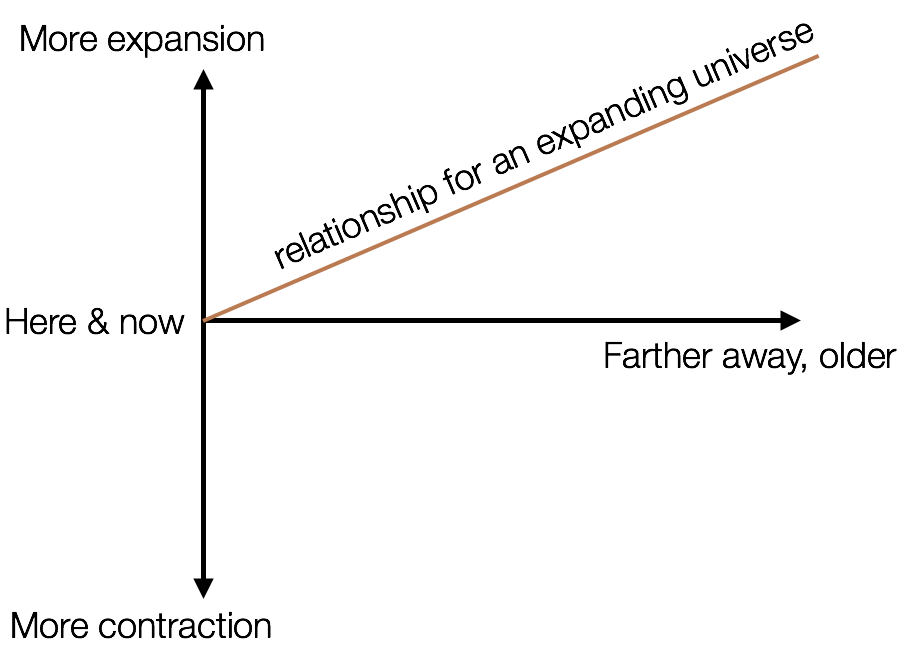
\includegraphics[width=0.5\textwidth]{hubble-diagram/hubble-diagram-schematic}
	\caption{Schematic of a Hubble diagram plot. It illustrates the relationship between the expansion
		experienced by a photon and the distance of its emitter.}\label{hd:fig:hubble-diagram-schematic}
\end{figure}

\begin{steps}
	\item\label{hd:step:sketch} Sketch the plot from Figure~\ref{hd:fig:hubble-diagram-schematic}, then sketch on the plot two more lines corresponding to the
	relationship for 1) a contracting universe, and 2) a static universe.
\end{steps}

From this relationship, we can determine whether the universe is
expanding, contracting, or static by looking at a number of galaxies and
measuring their distance (corresponding to the horizontal axis) and the
expansion experienced by their photons (corresponding to the vertical axis).

For this lab, we will use galaxy images and spectra listed in an online
table.

\section{Measuring distance}

We will use geometry to measure the distance of our galaxies. Galaxies
that are closer will look bigger and will subtend a larger angle whereas
galaxies that are further will looks smaller and will subtend a smaller
angle. This relationship between the angular size of the galaxy and its
distance is illustrated in Figure~\ref{hd:fig:galaxy-subtend}.

\begin{figure}
	\centering
	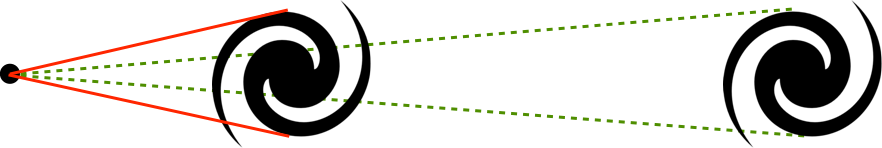
\includegraphics[width=\textwidth]{hubble-diagram/galaxy-subtend}
	\caption{Looking from the dot on the left, there are two galaxies that are the same size, one further away than the other. The more distant galaxy subtends a smaller angle (dashed green lines) than the closer galaxy (solid red lines).}\label{hd:fig:galaxy-subtend}
\end{figure}

Our galaxies will all be nearly the same size (22 kpc). Using the
geometry shown in the illustration, we can arrive at the following
relationship:
\begin{equation}\label{hd:eq:size}
 \textrm{angular size} = \frac{22\:\textrm{kpc}}{\textrm{distance}} \,.
\end{equation}
So, by measuring the angular size of our galaxy images, we can use the
above equation to determine the distance to the galaxy.

From the Modules $>$ Lab section of the Canvas site, download and extract to a folder \texttt{HubbleDataWebpage.zip}. In that folder, open \texttt{HubbleDataPage.html}. You
will find a list of galaxy names. Click on the ``Image'' link for the first
galaxy, NGC 1357. In the new tab, you will see an image of galaxy NGC
1357 similar to Figure~\ref{hd:fig:galaxy-example}.

\begin{figure}
	\centering
	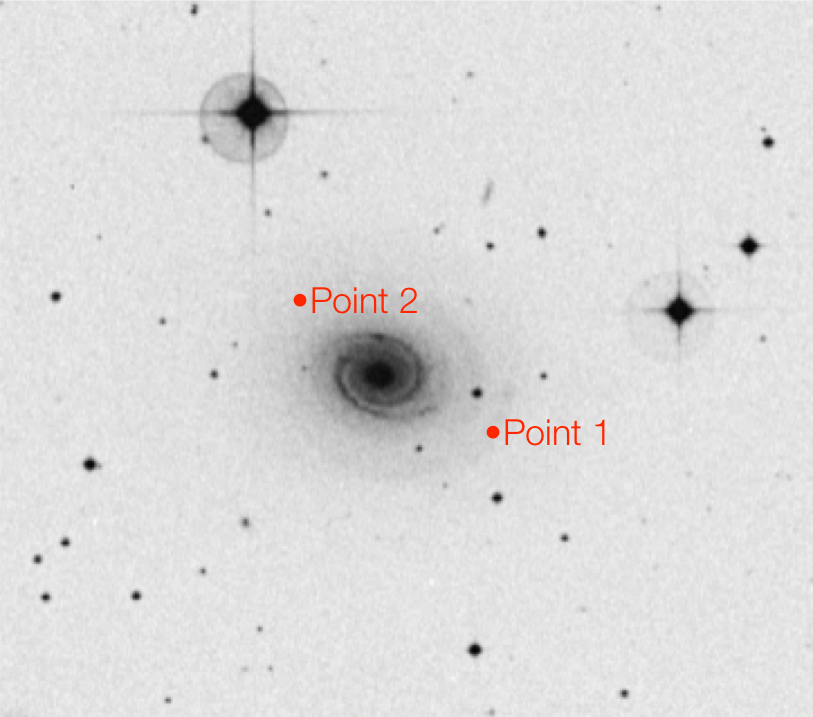
\includegraphics[width=0.5\textwidth]{hubble-diagram/galaxy-example}
	\caption{Example of galaxy image. Colors are inverted here, and Points 1 and 2 mark the furthest extent of the galaxy}\label{hd:fig:galaxy-example}
\end{figure}

\begin{steps}
	\item\label{hd:step:kind} What kind of galaxy is it (spiral, elliptical, unclear)? Note this in your spreadsheet.
	
	\item Are there any noteworthy features in the image? Use your spreadsheet to record your answers.
\end{steps}

We want to measure the angular size of NGC 1357, which you can do by
measuring the angular separation between two appropriate points
spanning the entire galaxy. In the lower left hand corner of google
skymaps, google shows you the coordinates of your cursor. Record the
coordinates (RA and DEC) for two points spanning the galaxy. Then use
an online calculator (e.g.
\url{http://cads.iiap.res.in/tools/angularSeparation}) to calculate the
angular separation between the points. Be careful and make sure that you don’t choose points that are too far
outside or inside the galaxy image.

\begin{steps}
	\item\label{hd:step:size} Enter the value for the angular size
(in radians, not degrees) in a spreadsheet.

	\item Divide up the remaining galaxy images between your groupmates
	and repeat Steps~\ref{hd:step:kind}--\ref{hd:step:size} for each of the galaxies recording your notes
	and measurements in the spreadsheet.
	
	\item Once you have measured the angular size of all the galaxies, use Equation~\ref{hd:eq:size} to estimate the distance for each galaxy
	and record the values in a “distance” column.
\end{steps}





\section{Measuring expansion}

The wavelength of light changes as the universe expands, an effect
known as cosmological redshifting. If the universe expands, the
wavelength is stretched, becoming longer and redder. For a contracting
universe, the wavelength will be compressed becoming bluer. We define
the redshift, $z$, as
\begin{equation}\label{hd:eq:redshift}
 z = \frac{\lambda_\textrm{measured} - \lambda_\textrm{original}}{\lambda_\textrm{original}} \,,
\end{equation}
where $\lambda$ represents the wavelength. The redshift is a measure of how much the wavelength has been
stretched or compressed.

We can measure the redshift by examining spectra (the energy emitted
in different wavelengths) of the same galaxies we just measured. For
NGC 1357, click on the link “Ca Spectra.” The link will show spectra
associated with Ca absorption which produces dips at wavelengths of
3933.7 angstroms and 3968.5 angstroms. You should see two
prominent dips in the data. See Figure~\ref{hd:fig:spectra} for example spectra.

\begin{figure}
	\centering
	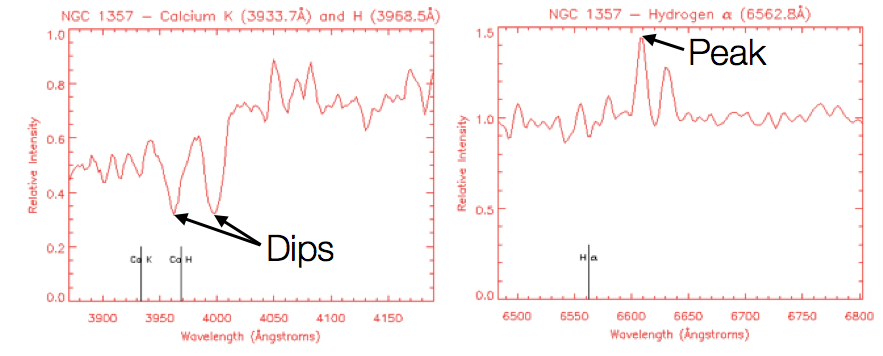
\includegraphics[width=\textwidth]{hubble-diagram/spectra}
	\caption{Spectrum of light detected from NGC 1357. The dips and peak that you will use to identify redshift are identified.}\label{hd:fig:spectra}
\end{figure}

Go back to the galaxy list and click on the
link “H-alpha spectrum” to bring up the spectra associated with
Hydrogen alpha emission of light with wavelength 6562.8 Angstroms.
You should see a clear peak in the data. The H-alpha peak is the leftmost
of the distribution. Since we know the original wavelengths for these
processes, we can compare the measured wavelength of these features
with their original wavelength to determine how much the light has
stretched.

\begin{steps}
	\item For each of the spectra estimate the value for the two Ca dips and the H-alpha peak. Record the values for the two Ca absorption lines and the H-alpha emission line in the excel worksheet. 
	
	\item Use Equation~\ref{hd:eq:redshift} to calculate the redshift for each of the lines and take the average to
estimate the redshift for the galaxy. Record the redshift in an “average
redshift” column in the spreadsheet.

	\item Repeat this process for each of
your galaxies.
\end{steps}

%\section{Compare your measurements}
%
%Compile the data between you and your groupmates into a single table.
%Compare your values for distance and redshift with those obtained by
%other groups in your section.
%
%\begin{steps}
%	\item How well do your data agree?
%	
%	\item Are they consistently different? If so, what do you think leads to
%	this discrepancy?
%	
%	\item Do they differ in a random fashion? If so, do they differ a lot or a
%	little? Provide your reasoning for your assessment.
%\end{steps}

\section{The Hubble diagram}

\begin{steps}
	
	\item Using the measurements in your worksheet, make a plot of redshift
	versus distance for your galaxies.
	
	\item Is there a trend in your data? Is the trend clear?
	
	\item Compare your plot with the sketches from Step~\ref{hd:step:sketch}. Does your data
	indicate that the universe is expanding? Contracting? Static? Why?

\end{steps}

Hubble's constant $H_0$ gives a relation between the recessional speed $v$ of an object and its distance $D$, according to the equation
\begin{equation}\label{hd:eq:hubble}
 v = H_0 D \,.
\end{equation}
You will determine Hubble's constant from your data. You have the distances of the galaxies already. To find the velocities, multiply the redshift by the speed of light $c$,
\begin{equation}
 v = zc \,.
\end{equation}
This equation is valid for low values of redshift.

\begin{steps}
	
	\item Make a Hubble diagram by plotting velocity (in km/s) vs. distance (in Mpc).
	
	\item Use this plot and Equation~\ref{hd:eq:hubble} to fit a line to the data and find Hubble's constant, which should be the slope of that line. If you are doing a linear fit, you need to force the $y$-intercept of the line to be zero. You may also need to specify that the fit equation be displayed on the plot.
	
	\item Do some research on the history and background of Hubble’s
	measurement. Write a one paragraph summary of this lab and discuss
	the following:
	\begin{enumerate}
		\item What was the historical context of Hubble’s measurement?
		\item Why was it important?
		\item What did you do in this lab and how do your measurements and
		conclusions compare with Hubble’s?
	\end{enumerate}
\end{steps}

\section{Report checklist and grading}

Each item below is worth 10 points.

\begin{enumerate}
	\item Data table
	
	\item Sketch of predicted relations for expanding, contracting, and static universes
	
	\item Your Hubble diagram (velocity vs. distance)
	
	\item Your Hubble constant
	
	\item Answers to Questions 11 and 15.
	
	\item A 100--200 word reflection on group dynamics and feedback on the lab manual. Address the following topics: who did what in the lab, how did you work together, what successes and challenges in group functioning did you have, and what would you keep and change about the lab write-up?
\end{enumerate}